% !TEX TS-program = pdflatex
% !TEX encoding = Isolatin

% Copyright Marius Hofert, Markus Kohm
% changed by D. Hennig, IT-Service ETH

%% Version 1.4 09.05.2011
%% !TEX TS-program = pdflatex
% !TEX encoding = Isolatin
% !TeX root = ..\ETH_praesentation.tex


%% Version 1.2 21.04.2011
% ==== class ===================================================================
\documentclass[
	paper=128mm:96mm,  % like beamer
	fontsize=11pt,     % like beamer
	pagesize,          % write page size to dvi or pdf
	parskip=half-,     % paragraphs are separated by half a line, no special marking of line
                       % endings
	numbers=noendperiod,% removes points for special parts (e.g. appendix)
	captions=nooneline % do not distinguish between one or more lines in captions
    ]{scrartcl}
\linespread{1.12}% enlarge line space
% ==== packages ================================================================

% font stuff
\usepackage[T1]{fontenc}% for correct hyphenation and T1 encoding
\AfterFile{t1lmss.fd}{  % see http://www.komascript.de/node/823
  \DeclareFontShape{T1}{lmss}{b}{n}
  {<->ssub*lmss/bx/n}{}
}
\usepackage{lmodern}        % latin modern font
\renewcommand{\familydefault}{\sfdefault}
\usepackage{helvet}         % helvetica as the origin of arial
\usepackage[helvet]{./ETH_res/sfmath} % for the mathematical enviroments
\usepackage{microtype}      % for character protrusion and font expansion (only with pdflatex)

% colors
\usepackage{xcolor}         % color package; load before tocstyle
\usepackage{wallpaper}      % background picture
\setlength{\wpXoffset}{0mm}
\setlength{\wpYoffset}{-10mm}

% page structure
\usepackage{calc}% working with lengths, counters etc.
\usepackage[includeheadfoot,
            top=-0.5mm, bottom=3.5mm,
            left=5.5mm, right=5.5mm,
            headsep=10.5mm, footskip=4.5mm]{geometry}% set page layout parameters
\usepackage{scrpage2}% package for page style with not only uppercase letters in the head
\usepackage{titlesec}% for reducing space between ((sub)sub)sections and text
\usepackage{tocstyle}% for adjusting table of contents
% === toc style ===
\makeatletter
    \newtocstyle[noonewithdot]{nodotnopagenumber}{
    % define tocstyle without dots and page numbers
            \settocfeature{pagenumberbox}{\@gobble}
    }
\makeatother
\usetocstyle{nodotnopagenumber}

% misc
\usepackage{amsthm}     % theorem environments
\usepackage{bm}         % for bold math symbols
\usepackage{enumitem}   % for automatic numbering of new enumerate environments
\usepackage{graphicx}   % for including figures
%\graphicspath{{pictures/}}

\usepackage{tikz}       % sophisticated graphics package
\usepackage{tabularx}   % for special table environment (tabularx-table)
\usepackage{booktabs}   % for table layout
\usepackage{natbib}     % for bibliography with astron-style
\bibliographystyle{astron}
\usepackage{siunitx}    % to use for international units in the real world

\usepackage[
    hypertexnames=false,% for correct links (duplicate-error solution)
	setpagesize=false,  % necessary in order to not change text-/paperformat for the document
	pdfborder={0 0 0},  % removes border around links
	pdfpagemode=FullScreen,% open pdf in full screen mode
    pdfstartview=Fit    % fit page to pdf viewer
]{hyperref}% all links stay black and are thus invisible
%\hypersetup{% Note: If \ETHauthor or \ETHtitle contain non-us-ascii-chars you
%            % should not use them inside \hyperref.
%  pdfauthor=\ETHauthor,
%  pdftitle=\ETHtitle
%}  % docymentsyle and packages
% !TEX TS-program = pdflatex
% !TEX encoding = Isolatin
% !TeX root = ..\ETH_praesentation.tex


%% Version 1.2 21.04.2011
% ==== class ===================================================================
\documentclass[
	paper=128mm:96mm,  % like beamer
	fontsize=11pt,     % like beamer
	pagesize,          % write page size to dvi or pdf
	parskip=half-,     % paragraphs are separated by half a line, no special marking of line
                       % endings
	numbers=noendperiod,% removes points for special parts (e.g. appendix)
	captions=nooneline % do not distinguish between one or more lines in captions
    ]{scrartcl}
\linespread{1.12}% enlarge line space
% ==== packages ================================================================

% font stuff
\usepackage[T1]{fontenc}% for correct hyphenation and T1 encoding
\AfterFile{t1lmss.fd}{  % see http://www.komascript.de/node/823
  \DeclareFontShape{T1}{lmss}{b}{n}
  {<->ssub*lmss/bx/n}{}
}
\usepackage{lmodern}        % latin modern font
\renewcommand{\familydefault}{\sfdefault}
\usepackage{helvet}         % helvetica as the origin of arial
\usepackage[helvet]{./ETH_res/sfmath} % for the mathematical enviroments
\usepackage{microtype}      % for character protrusion and font expansion (only with pdflatex)

% colors
\usepackage{xcolor}         % color package; load before tocstyle
\usepackage{wallpaper}      % background picture
\setlength{\wpXoffset}{0mm}
\setlength{\wpYoffset}{-10mm}

% page structure
\usepackage{calc}% working with lengths, counters etc.
\usepackage[includeheadfoot,
            top=-0.5mm, bottom=3.5mm,
            left=5.5mm, right=5.5mm,
            headsep=10.5mm, footskip=4.5mm]{geometry}% set page layout parameters
\usepackage{scrpage2}% package for page style with not only uppercase letters in the head
\usepackage{titlesec}% for reducing space between ((sub)sub)sections and text
\usepackage{tocstyle}% for adjusting table of contents
% === toc style ===
\makeatletter
    \newtocstyle[noonewithdot]{nodotnopagenumber}{
    % define tocstyle without dots and page numbers
            \settocfeature{pagenumberbox}{\@gobble}
    }
\makeatother
\usetocstyle{nodotnopagenumber}

% misc
\usepackage{amsthm}     % theorem environments
\usepackage{bm}         % for bold math symbols
\usepackage{enumitem}   % for automatic numbering of new enumerate environments
\usepackage{graphicx}   % for including figures
%\graphicspath{{pictures/}}

\usepackage{tikz}       % sophisticated graphics package
\usepackage{tabularx}   % for special table environment (tabularx-table)
\usepackage{booktabs}   % for table layout
\usepackage{natbib}     % for bibliography with astron-style
\bibliographystyle{astron}
\usepackage{siunitx}    % to use for international units in the real world

\usepackage[
    hypertexnames=false,% for correct links (duplicate-error solution)
	setpagesize=false,  % necessary in order to not change text-/paperformat for the document
	pdfborder={0 0 0},  % removes border around links
	pdfpagemode=FullScreen,% open pdf in full screen mode
    pdfstartview=Fit    % fit page to pdf viewer
]{hyperref}% all links stay black and are thus invisible
%\hypersetup{% Note: If \ETHauthor or \ETHtitle contain non-us-ascii-chars you
%            % should not use them inside \hyperref.
%  pdfauthor=\ETHauthor,
%  pdftitle=\ETHtitle
%}  % docymentsyle and packages
%% !TEX TS-program = pdflatex
% !TEX encoding = Isolatin
% !TeX root = ..\ETH_praesentation.tex


%% Version 1.2 21.04.2011
% ==== settings page style and foot ============================================
\pagestyle{scrheadings} % activates pagestyle from scrpage2
\clearscrheadfoot       % clear head and foot of scrheadings and scrplain
                        % setting for page head and foot
\setkomafont{pageheadfoot}{\normalfont\color{black}\sffamily}
% optical vertical centering of page contents
\makeatletter
    \renewcommand*{\@textbottom}{\vskip \z@ \@plus 1fil}
    \newcommand*{\@texttop}{\vskip \z@ \@plus .5fil}
    \addtolength{\parskip}{\z@\@plus .25fil}% stretch parskip a lot
\makeatother
% ==== head ====================================================================
\setheadwidth[0pt]{textwithmarginpar}
\clearscrheadfoot
% head (optional argument is scrplain, mandatory scrheadings)
\lohead{\begin{minipage}[t]{40mm}
              \vspace{0mm}
              
\includegraphics[width=0.7\textwidth]{ETH_res/ETH_logo.pdf}
        \end{minipage}
}%

\rohead{\begin{minipage}[t]{35.5mm}
               \vspace*{-1mm}\renewcommand{\baselinestretch}{0.4}
               \bf
               \fontsize{8}{9}\selectfont
               \ETHdeptshort\\\\
               \fontsize{4}{5}\selectfont
               \ETHdeptlong\\
               \ETHinstitut
               \end{minipage}
        }
% ==== foot ====================================================================
\newlength{\footheight}
\setlength{\footheight}{6mm}
\setkomafont{pagefoot}{\normalfont\sffamily\color{white}}
\addtokomafont{pagefoot}{\tiny}% general setting for the foot
\setkomafont{pagenumber}{\color{white}}% setting for page foot
\ifoot{% foot inside (left) to include the figur
	\hspace{-6.0mm}
    \vspace{-8.5mm}
	\begin{tikzpicture}[remember picture,overlay]
		\node [xshift=\paperwidth/2,yshift=\footheight/2]
        {
\includegraphics[width=\paperwidth]{ETH_res/ETH_footer.jpg}};
	\end{tikzpicture}%
}%

\cfoot{% foot center to include the text
    \ifnum\value{page} > 1            % first page without footer writings
        \vspace{-6.5mm}
        {\fontsize{5}{6}\selectfont   % very small font
            \begin{minipage}[b]{50mm} % left
                \ETHdate
            \end{minipage}
            \begin{minipage}[b]{57mm} % center
                \ETHauthor
            \end{minipage}
            \begin{minipage}[b]{8mm}  % right
                \hfill \pagemark
            \end{minipage}
        }
    \fi
}%
% ==== end settings page style and foot ========================================

% theorems, proofs
\newtheoremstyle{ETHthmstyle}%
	{0.5em}% space above
	{0.5em}% space below
	{}% body font
	{}% indent amount
	{\sffamily\bfseries}% head font
	{}% punctuation after head
	{\newline}% space after head
	{\thmname{#1}\ \thmnote{(#3)}}% head spec
\theoremstyle{ETHthmstyle}
\newtheorem{theorem}{Theorem}[section]
\newtheorem{remark}[theorem]{Remark}
\newtheorem{algorithm}[theorem]{Algorithm}
\renewcommand*\proofname{Proof}
\makeatletter% correct qed adjustment
    \renewenvironment{proof}[1][\proofname]{\par
    \pushQED{\qed}
    \normalfont\topsep2\p@\@plus2\p@\relax
    \trivlist
    \item[\hskip\labelsep
	      \sffamily\bfseries #1]\mbox{}\hfill\\*\ignorespaces
          }{\popQED\endtrivlist\@endpefalse
    }
\makeatother
% note environment
\newenvironment{note}[1]{
  \labeling{#1}
		\item[#1]\ignorespaces
    }{\endlabeling
    }

% ==== commands ================================================================

% decoration
\usetikzlibrary{decorations.pathmorphing,shadows}


% box
\newcommand*{\ETHbox}[2]{% width, content
	\par\noindent
	\begin{tikzpicture}[ETHnodestyle/.style={rectangle,rounded
            corners,draw=ETHdarkgray!40!white,
            thick,inner sep=2mm,text justified,top color=ETHlightblue!30!white, bottom color=ETHlightblue,above}]%
		    \node[ETHnodestyle,at={(0.5*#1+2mm+0.4pt,0)}]{%
			\begin{minipage}[t]{#1}
				#2
			\end{minipage}%
		    };
%		    \node[ETHnodestyle,at={(0.5*#1+2mm+0.4pt,-0.1)},yscale=-0.33,scope
%                  fading=south,opacity=0.85]{%
%			     \begin{minipage}[t]{#1}
%				        \strut
%			     \end{minipage}%
%		          };
	\end{tikzpicture}%	
	\par\vspace{-1.3em}
}

% labels
\newcommand*{\ETHitem}{\raisebox{1pt}{\tikz\fill[sharp
    corners](0,0)rectangle+(3.4pt,3.4pt);}}

% spacings & make the title section fonts slightly smaller
\titleformat{\section}{\large\bfseries}{\thesection}{1em}{}
\titlespacing{\section}{0mm}{0mm}{0mm}
% make space (left, before, after) between section and text smaller
\titlespacing{\subsection}{0mm}{0mm}{-1mm}
% make space (left, before, after) between subsection and text smaller
\titlespacing{\subsubsection}{0mm}{0mm}{-2mm}
% make space (left, before, after) between subsubsection and text smaller
\setcounter{secnumdepth}{2}% add numbering down to subsection  % settings
% !TEX TS-program = pdflatex
% !TEX encoding = Isolatin
% !TeX root = ..\ETH_praesentation.tex


%% Version 1.2 21.04.2011
% ==== settings page style and foot ============================================
\pagestyle{scrheadings} % activates pagestyle from scrpage2
\clearscrheadfoot       % clear head and foot of scrheadings and scrplain
                        % setting for page head and foot
\setkomafont{pageheadfoot}{\normalfont\color{black}\sffamily}
% optical vertical centering of page contents
\makeatletter
    \renewcommand*{\@textbottom}{\vskip \z@ \@plus 1fil}
    \newcommand*{\@texttop}{\vskip \z@ \@plus .5fil}
    \addtolength{\parskip}{\z@\@plus .25fil}% stretch parskip a lot
\makeatother
% ==== head ====================================================================
\setheadwidth[0pt]{textwithmarginpar}
\clearscrheadfoot
% head (optional argument is scrplain, mandatory scrheadings)
\lohead{\begin{minipage}[t]{40mm}
              \vspace{0mm}
              %
\includegraphics[width=0.7\textwidth]{ETH_res/ETH_logo.pdf}
              
\includegraphics[width=0.7\textwidth]{ETH_logo.pdf}
        \end{minipage}
}%

\rohead{\begin{minipage}[t]{35.5mm}
               \vspace*{-1mm}\renewcommand{\baselinestretch}{0.4}
               \bf
               \fontsize{8}{9}\selectfont
               \ETHdeptshort\\\\
               \fontsize{4}{5}\selectfont
               \ETHdeptlong\\
               \ETHinstitut
               \end{minipage}
        }
% ==== foot ====================================================================
\newlength{\footheight}
\setlength{\footheight}{6mm}
\setkomafont{pagefoot}{\normalfont\sffamily\color{white}}
\addtokomafont{pagefoot}{\tiny}% general setting for the foot
\setkomafont{pagenumber}{\color{white}}% setting for page foot
\ifoot{% foot inside (left) to include the figur
	\hspace{-6.0mm}
    \vspace{-8.5mm}
	\begin{tikzpicture}[remember picture,overlay]
		\node [xshift=\paperwidth/2,yshift=\footheight/2]
%        {
\includegraphics[width=\paperwidth]{ETH_res/ETH_footer.jpg}};
        {
\includegraphics[width=\paperwidth]{ETH_footer.jpg}};
	\end{tikzpicture}%
}%

\cfoot{% foot center to include the text
    \ifnum\value{page} > 1            % first page without footer writings
        \vspace{-6.5mm}
        {\fontsize{5}{6}\selectfont   % very small font
            \begin{minipage}[b]{50mm} % left
                \ETHdate
            \end{minipage}
            \begin{minipage}[b]{57mm} % center
                \ETHauthor
            \end{minipage}
            \begin{minipage}[b]{8mm}  % right
                \hfill \pagemark
            \end{minipage}
        }
    \fi
}%
% ==== end settings page style and foot ========================================

% theorems, proofs
\newtheoremstyle{ETHthmstyle}%
	{0.5em}% space above
	{0.5em}% space below
	{}% body font
	{}% indent amount
	{\sffamily\bfseries}% head font
	{}% punctuation after head
	{\newline}% space after head
	{\thmname{#1}\ \thmnote{(#3)}}% head spec
\theoremstyle{ETHthmstyle}
\newtheorem{theorem}{Theorem}[section]
\newtheorem{remark}[theorem]{Remark}
\newtheorem{algorithm}[theorem]{Algorithm}
\renewcommand*\proofname{Proof}
\makeatletter% correct qed adjustment
    \renewenvironment{proof}[1][\proofname]{\par
    \pushQED{\qed}
    \normalfont\topsep2\p@\@plus2\p@\relax
    \trivlist
    \item[\hskip\labelsep
	      \sffamily\bfseries #1]\mbox{}\hfill\\*\ignorespaces
          }{\popQED\endtrivlist\@endpefalse
    }
\makeatother
% note environment
\newenvironment{note}[1]{
  \labeling{#1}
		\item[#1]\ignorespaces
    }{\endlabeling
    }

% ==== commands ================================================================

% decoration
\usetikzlibrary{decorations.pathmorphing,shadows}


% box
\newcommand*{\ETHbox}[2]{% width, content
	\par\noindent
	\begin{tikzpicture}[ETHnodestyle/.style={rectangle,rounded
            corners,draw=ETHdarkgray!40!white,
            thick,inner sep=2mm,text justified,top color=ETHlightblue!30!white, bottom color=ETHlightblue,above}]%
		    \node[ETHnodestyle,at={(0.5*#1+2mm+0.4pt,0)}]{%
			\begin{minipage}[t]{#1}
				#2
			\end{minipage}%
		    };
%		    \node[ETHnodestyle,at={(0.5*#1+2mm+0.4pt,-0.1)},yscale=-0.33,scope
%                  fading=south,opacity=0.85]{%
%			     \begin{minipage}[t]{#1}
%				        \strut
%			     \end{minipage}%
%		          };
	\end{tikzpicture}%	
	\par\vspace{-1.3em}
}

% labels
\newcommand*{\ETHitem}{\raisebox{1pt}{\tikz\fill[sharp
    corners](0,0)rectangle+(3.4pt,3.4pt);}}

% spacings & make the title section fonts slightly smaller
\titleformat{\section}{\large\bfseries}{\thesection}{1em}{}
\titlespacing{\section}{0mm}{0mm}{0mm}
% make space (left, before, after) between section and text smaller
\titlespacing{\subsection}{0mm}{0mm}{-1mm}
% make space (left, before, after) between subsection and text smaller
\titlespacing{\subsubsection}{0mm}{0mm}{-2mm}
% make space (left, before, after) between subsubsection and text smaller
\setcounter{secnumdepth}{2}% add numbering down to subsection  % settings

% ====  colors  ================================================================
\definecolor{ETHblue}{RGB}{51,89,148}           % #335994
\definecolor{ETHlightblue}{RGB}{114,129,192}    % for Department-Logo
\definecolor{ETHtitleblue}{RGB}{0,49,91}        % for title (#00315b)
\definecolor{ETHbrown}{RGB}{148,116,51}
\definecolor{ETHred}{RGB}{161,82,71}
\definecolor{ETHdarkgray}{rgb}{0.282,0.322,0.361}    % for box (#48525c)
\definecolor{ETHlightgray}{RGB}{211,211,211}
\newcommand*{\ETHblue}[1]{\textcolor{ETHblue}{#1}} %for faint text
\newcommand*{\ETHlightblue}[1]{\textcolor{ETHlightblue}{#1}}
\newcommand*{\ETHtitleblue}[1]{\textcolor{ETHtitleblue}{#1}}
\newcommand*{\ETHbrown}[1]{\textcolor{ETHbrown}{#1}}
\newcommand*{\ETHred}[1]{\textcolor{ETHred}{#1}}
\newcommand*{\ETHdarkgray}[1]{\textcolor{ETHdarkgray}{#1}}

% ==== document related info ===================================================
\newcommand*{\ETHdeptshort}{\textsc {\color{ETHlightblue}D}\,MATH}
\newcommand*{\ETHdeptlong}{Department of Mathematics}
\newcommand*{\ETHinstitut}{Seminar for Statistics}
\newcommand*{\ETHtitle}{Student Seminar: Causality}
\newcommand*{\ETHsubtitle}{VIII Non-parametric Independence Test }
\newcommand*{\ETHauthor}{Dan MacKinlay, Clara Pelloni, Ambra Toletti}
\newcommand*{\ETHdate}{Monday, 29th April 2013}

% ==== document language =======================================================
% American English
\usepackage[american]{babel}
%\selectlanguage{american}

% we want these for nice mathematical typesetting
\usepackage{amssymb,amsmath}
\usepackage{amsthm}
\usepackage{bbm}
\usepackage{mathtools}
\usepackage{wrapfig}
\usepackage{rotating}
%fix horrible outline formatting
\usepackage[shortcuts]{extdash}

\newtheorem*{defn}{Definition}
\newtheorem*{fact}{Fact}


\DeclareMathOperator*{\corr}{corr}
\DeclareMathOperator*{\HSIC}{HSIC}

\setcounter{tocdepth}{2}
\AtBeginDocument{\renewcaptionname{american}{\contentsname}{\large Outline}}% toc-name

% ==== document ================================================================
\begin{document}
% ==============================================================================
% titlepage 1
% background picture
\begin{tikzpicture}[overlay]
    \node [shift={(-69.5mm,-133.95mm)}]  at (current page.north east)
    %% ETH-Hauptgebaeude (main building of the ETH)
%    {
\includegraphics[width=\paperwidth]{ETH_res/ETH_HG.jpg}};
    {
\includegraphics[width=\paperwidth]{ETH_HG.jpg}};
\end{tikzpicture}%
% content title
\begin{flushright}
    %\vspace{-7mm}
    %{\bfseries\Large\ETHtitle\par}
\end{flushright}
	\vspace{-46.5mm}
	{\bfseries\Large{\color{ETHtitleblue}\ETHtitle}}\par
    \vspace{-3.5mm}
    \Large\ETHsubtitle
\clearpage
\vspace*{-16.5mm}
\tableofcontents
\clearpage
% ==============================================================================

%#### Please fill in your normal Latex document and add some clearpage-commands.
\section{What are we doing today?}

Presenting a non-parametric independence test.

Here are the steps

\begin{enumerate}
	\item Explain why we bother
	\item Present necessary functional analysis background,
	\item Actually derive the test (in two different ways), then,
	\item Construct estimator from data
\end{enumerate}

\clearpage

\section{Why we bother}

\begin{enumerate}
	\item Last week we saw the PC and IC algorithms for inferring the DAG \ldots 
	\item \ldots by estimating pairwise conditional independence\ldots
	\item \ldots from samples of the joint distribution \ldots
	\item \ldots using the \emph{partial correlation} test to infer conditional independence
\end{enumerate}
\clearpage
\dots but partial correlation algorithm only works for linearly additive, Gaussian noise.
\clearpage

Consider:
\begin{enumerate}
\item Categorical data \emph{(If it's raining/if the sprinkler is on/\ldots)}
\item Non-gaussian noise \emph{(e.g. exponential)}
\item Non-additive coupling \emph{(e.g. multiplicative)}
\item Whatever combination of exotic data types, noise and interactions that you would like\dots \emph{(Nucleotide sequences..?)}
\end{enumerate}
\clearpage
Even correlation between 2 $\mathbb{R}$-valued RVs has notorious shortcomings.

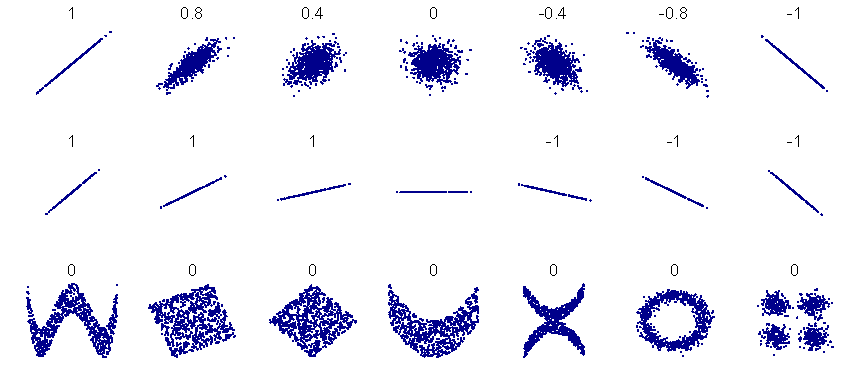
\includegraphics[width=\textwidth]{Correlation_examples2.pdf}
\clearpage
\subsection*{Some correlation test examples}
\clearpage
\begin{wrapfigure}{l}{0.5\textwidth}
  \begin{center}
    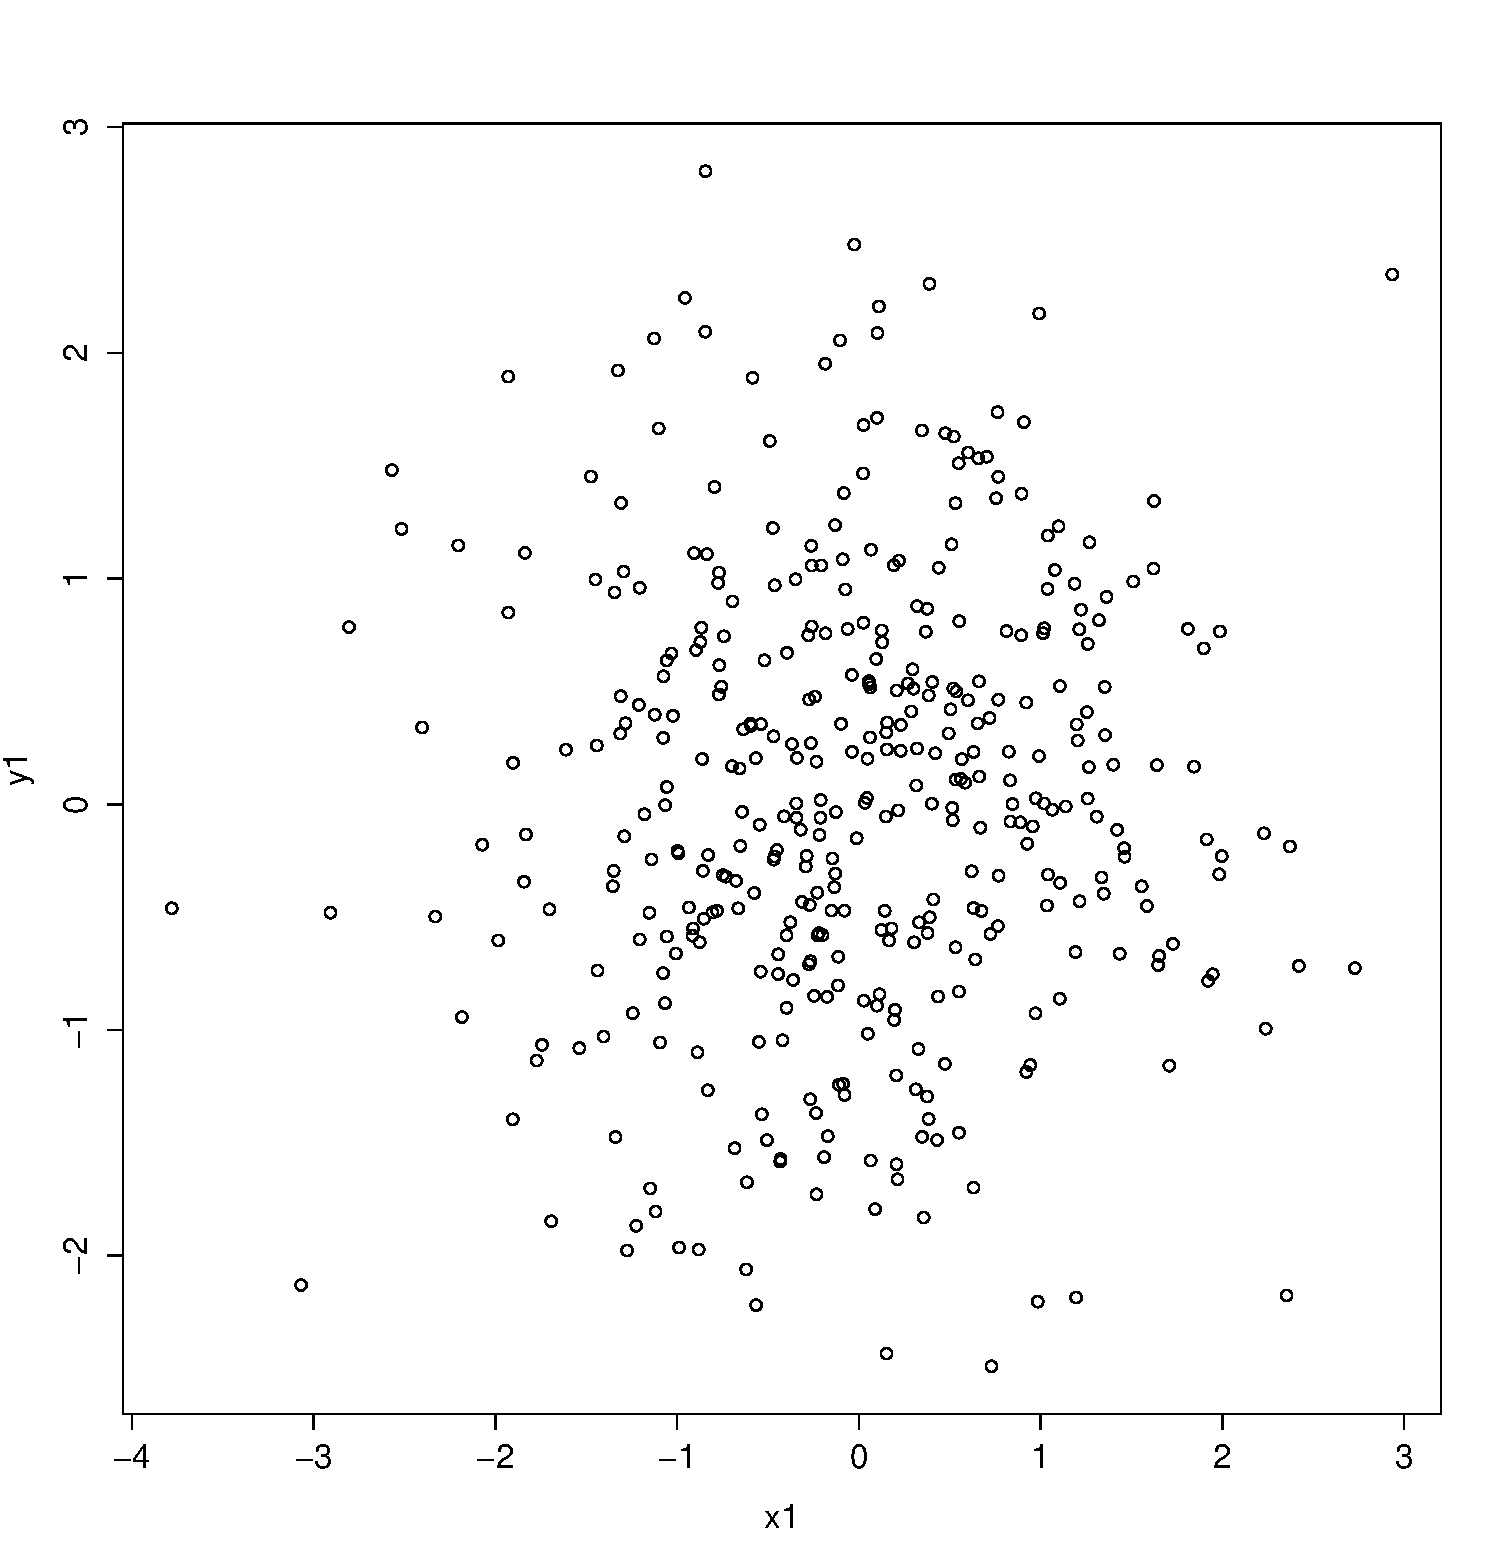
\includegraphics[width=5cm]{x1_vs_y1.pdf}
  \end{center}
\end{wrapfigure}
$H_0$: $\corr(x_1, y_1)=0$.

$H_A$: $\corr(x_1, y_1)\ne0$.

$P_0 = 0.23$

\clearpage
\begin{wrapfigure}{l}{0.5\textwidth}
  \begin{center}
    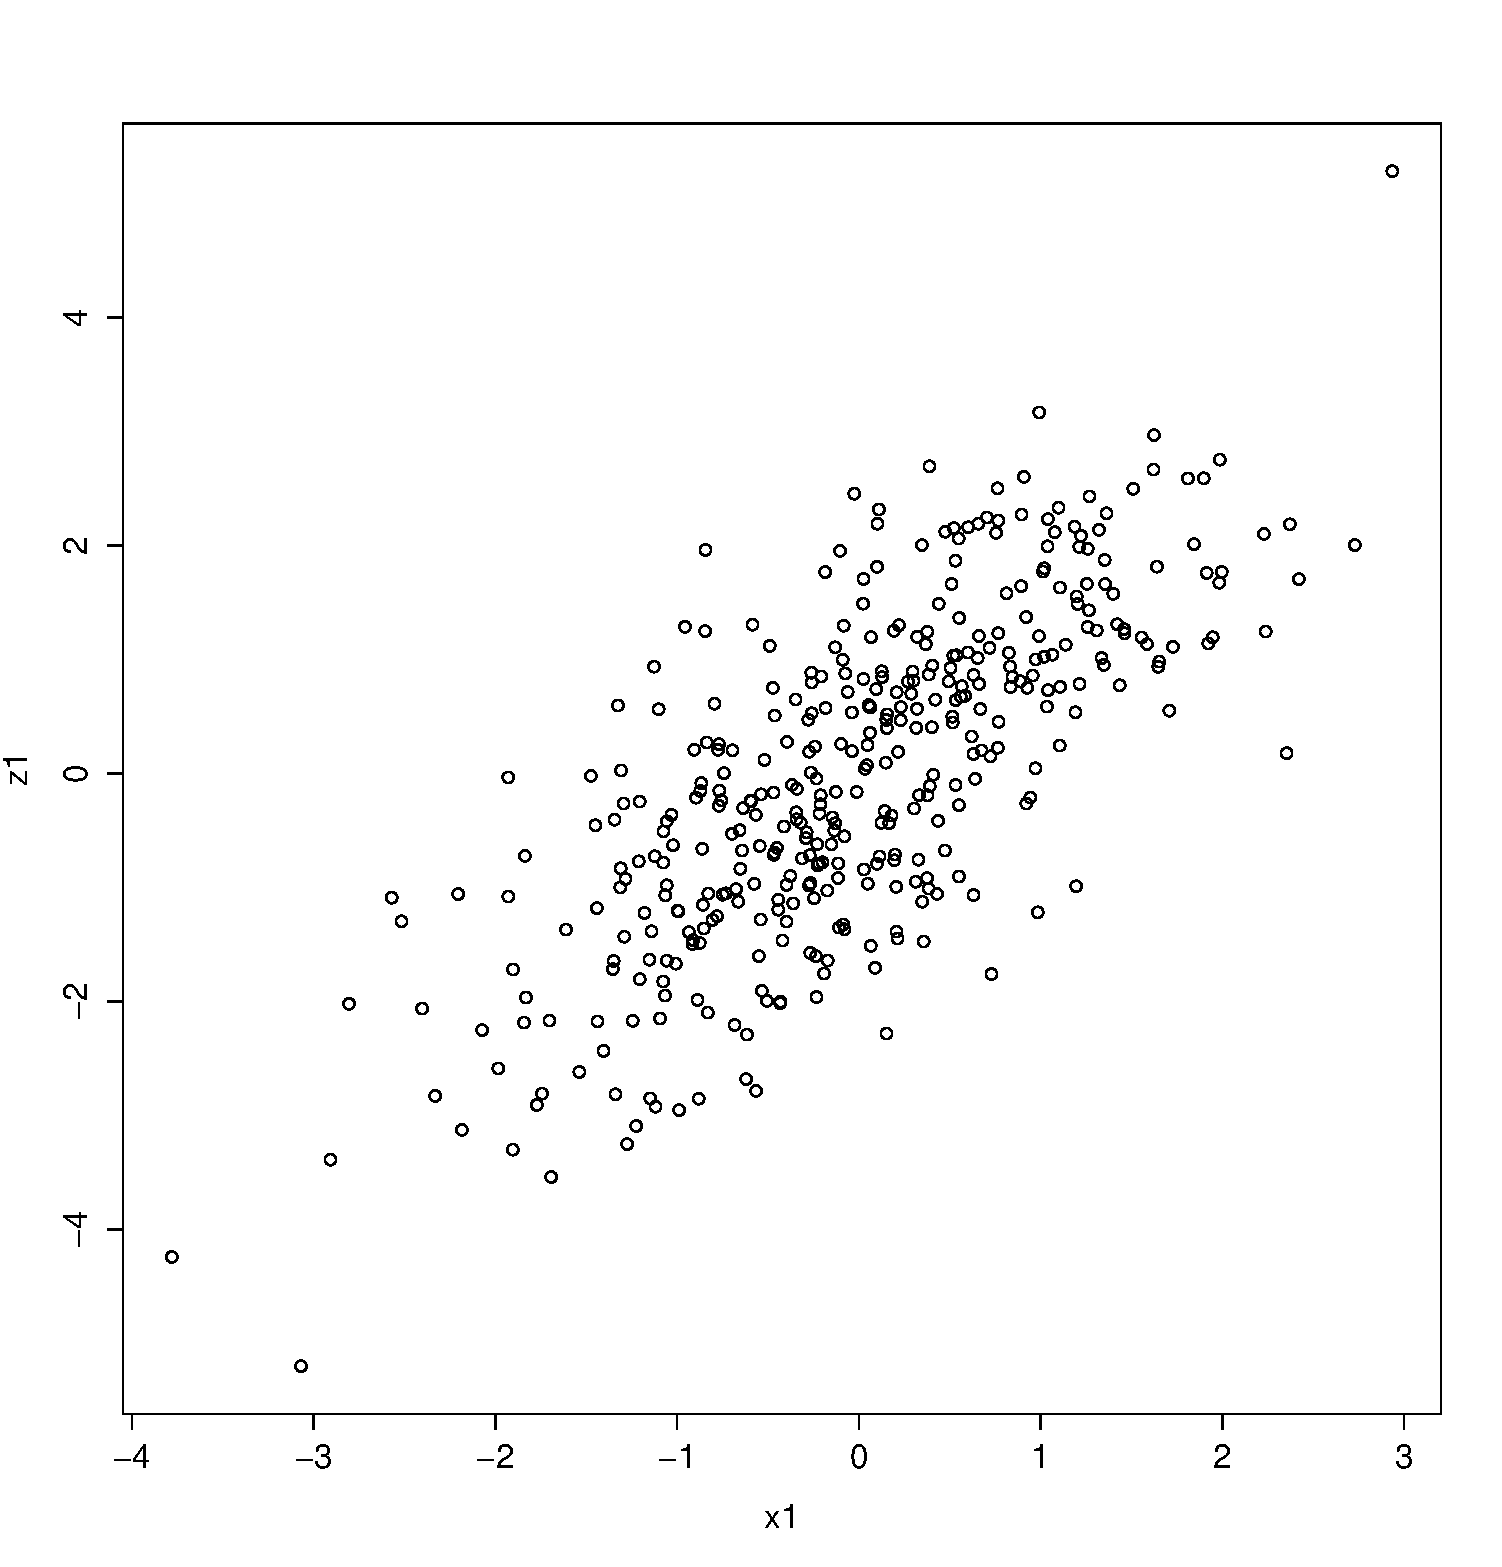
\includegraphics[width=5cm]{x1_vs_z1.pdf}
  \end{center}
\end{wrapfigure}
$H_0$: $\corr(x_1, z_1)=0$.

$H_A$: $\corr(x_1, z_1)\ne0$.

$P_0 = 0.0$
\clearpage
\begin{wrapfigure}{l}{0.5\textwidth}
  \begin{center}
    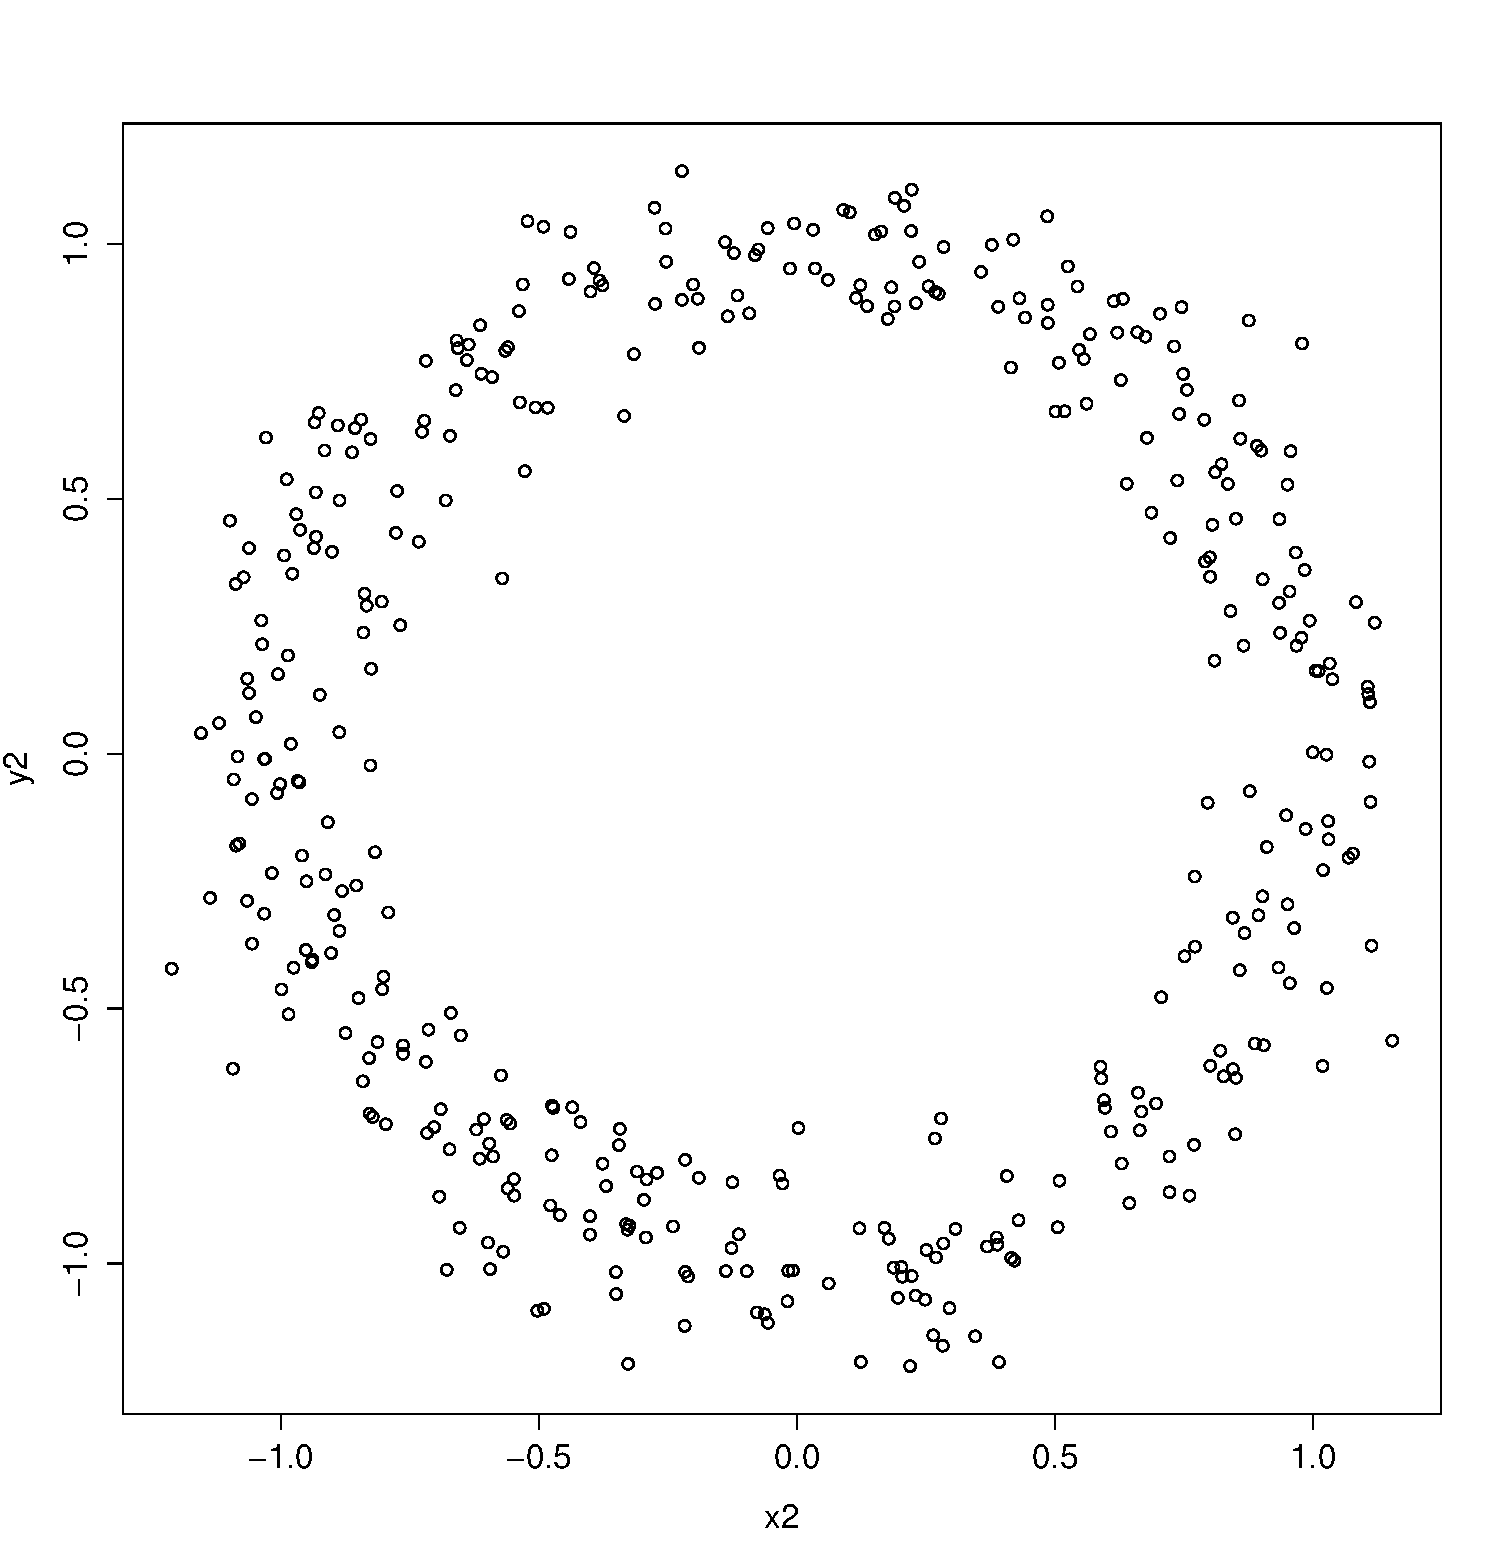
\includegraphics[width=5cm]{x2_vs_y2.pdf}
  \end{center}
\end{wrapfigure}
$H_0$: $\corr(x_1, z_1)=0.15$.

$H_A$: $\corr(x_1, z_1)\ne0$.

$P_0 = 0.15$
\clearpage

Therefore: More general tests are desirable.

Why not non-parametric tests?

\clearpage

What independence tests can relax the strong assumptions of partial correlation?

There are many! e.g. mutual information, rank statistics, copula measures\ldots

\clearpage
Today:

The \emph{Hilbert Schmidt Independence Criterion (HSIC)}

A ``kernelisation''-based~\footnote{as made famous by Support Vector Machines} method, has attractive features.
\begin{enumerate}
\item It can handle arbitrary input spaces, not just $\mathbb{R}^d$ (e.g. nucleotide strings, sprinkler settings)
\item It is natural to conditionalize.
\end{enumerate}
\clearpage
NB: Today we will only construct the marginal (unconditional) independence measure on $\mathcal{X}=\mathbb{R}^d$, by way of introduction. (Homework: conditional estimator on general input spaces.)

\clearpage
\section{Functional analysis in 15 minutes}
We want to transform our arbitrary data into a natural ``feature'' space with convenient representations of relations between data.

Functional analysis gives us the \emph{Hilbert space}, which formalises this.

\clearpage
\subsection*{The classic example}

    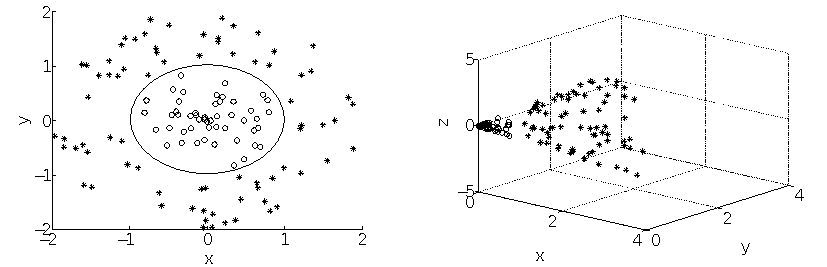
\includegraphics[width=\textwidth]{diploma_separation_diagrams.pdf}
    
    We want to separate 2 classes points in $\mathbb{R}^2$ (left) with a linear decision boundary. But we can't.
    
    We \emph{can} separate the ones in $\mathbb{R}^3$ on the right though.
 
 \clearpage
In fact, the ones on the right are a transformed version of the ones on the left, using a mapping:
\begin{equation*}
	\phi: \begin{matrix}
		\mathbb{R}^2  &\rightarrow &\mathbb{R}^3\\
		(x,y) &\mapsto &\left(x^2, y^2, \sqrt{2}xy\right)
	\end{matrix}
\end{equation*}

Can we find a general method for constructing such convenient transforms?
\clearpage
\subsection*{Making this general}

\begin{defn}
A Hilbert space $\mathcal{H}$ is a vector space with an inner product $\langle\cdot,\cdot\rangle: \mathcal{H}\times\mathcal{H} \rightarrow\mathbb{R}$.
\end{defn}

Additional technical requirement: It is \emph{complete}.

Bonus functional analysis ``twist'': It need \emph{not} be a finite dimensional vector space.
\clearpage
\begin{defn}
An \emph{inner product}, $\langle\cdot,\cdot\rangle$ on a Hilbert space generalises the definition on $\mathbb{R}^d$.

For $f,\,g$ and $h \in \mathcal{H}$ and for $\alpha$ and $\beta \in \mathbb{R}$:
\begin{enumerate}
\item $\langle\alpha f + \beta g, h\rangle = \alpha\langle f, h\rangle + \beta\langle g, h\rangle$
\item $\langle f, g\rangle = \langle g, f \rangle$
\item $\langle f, f \rangle \ge 0$ and $\langle f, f\rangle = 0$ iff $f =0$
\end{enumerate}
\end{defn}

\clearpage

So we have defined some operations in this feature space.

But our data does not come from such as space.

Let's consider the ``input'' space $\mathcal{X}\ne\mathcal{H}$, and points $x_i \in \mathcal{X}$ drawn from it.

We will use \emph{kernel} functions to relate them.
\clearpage
We define define a \emph{kernel}, $k$,
\begin{equation*}
k : \mathcal{X} \times \mathcal{X} \rightarrow \mathbb{R}
\end{equation*}
and a map
\begin{equation}
\phi: \mathcal{X} \rightarrow \mathcal{H}
\end{equation}
such that 
\begin{equation*}
k(x, x') = \langle \phi(x), \phi(x') \rangle
\end{equation*}
\clearpage
\begin{defn}
A function 
\begin{equation*}
k:\mathcal{X} \times \mathcal{X}\rightarrow \mathbb{R}
\end{equation*}
 is \emph{positive definite} if,
for all $n \ge 1$,
for all $(a_1, a_2, \ldots, a_n) \in \mathbb{R}^n$ and
for all $(x_1, x_2, \ldots, x_n) \in \mathcal{X}^n$,
\begin{equation*}
\sum_{i=1}^n\sum_{j=1}^n a_i a_j k(x_i, x_j) \ge 0
\end{equation*}
\end{defn}
\clearpage
\begin{fact}
Take $\mathcal{H}$ any Hilbert space, and 
\begin{equation*}
\phi: \mathcal{X} \rightarrow \mathcal{H}
\end{equation*}
Then  
\begin{equation*}
k(x, x') = \langle \phi(x), \phi(x') \rangle
\end{equation*}
is a positive definite function.
\end{fact}
But the converse also holds.
\clearpage
\begin{fact}
Take a positive definite function $k : \mathcal{X} \times \mathcal{X} \rightarrow \mathbb{R}$.
Then, there exists a Hilbert space $\mathcal{H}$, and mapping
\begin{equation*}
\phi: \mathcal{X} \rightarrow \mathcal{H}
\end{equation*}
 such that
 \begin{equation*}
 k(x, x') = \langle \phi(x), \phi(x') \rangle
 \end{equation*}
is a positive definite function.
\end{fact}
\clearpage
Therefore:

Given a kernel, we can use it calculate an inner-product between a transformed version of points $x \in \mathcal{X}$ in some \emph{implicit} Hilbert space.

Indeed, $\mathcal{H}$ can be strange indeed.
\clearpage
\subsection*{Reproducing Kernel Hilbert Space (RKHS)}
We impose some additional, useful structure.

Hilbert space of functions
\begin{equation*}
f: \mathcal{X} \rightarrow \mathbb{R}
\end{equation*}
 and 
\begin{equation*}
\forall x \in \mathcal{X}, k(\cdot, x) \in \mathcal{H}
\end{equation*}
(A space of functions \emph{on} $\mathcal{X}$.)
\clearpage
Moreover,  require the \emph{reproducing property}
\begin{align*}
\forall f \in \mathcal{H}, \forall x \in \mathcal{X},\\
\langle f, k(\cdot,x)\rangle = f(x)\rangle
\end{align*}
In such spaces we have that 
\begin{equation*}
k(x,y) = \langle k(\cdot, x), k(\cdot, y) \rangle
\end{equation*}
\clearpage
That is, our kernel $k$ induces the following $\phi$-mapping
\begin{equation*}
\phi: \begin{matrix}
        \mathcal{X}  &\rightarrow &\mathcal{H}\\
        x &\mapsto &k(x,\cdot)
        \end{matrix}
\end{equation*}
\clearpage
Example kernels on $x, y \in \mathbb{R}^d$
\begin{enumerate}
\item linear kernel \[k(x, y) = x^Ty\]
\item polynomial kernel of degree $d\in \mathbb{N}$: \[k(x, y) = (x^Ty)^d\]
\item Gaussian kernel of bandwidth $\sigma>0$, \[k(x,y) = \exp\left(-\frac{(x-y)^T(x-y)}{2\sigma^2}\right)\]
\end{enumerate}
\clearpage
We will use the Gaussian kernel again.

Nice, intuitive, properties for demonstration.

\begin{itemize}
\item \emph{translation invariant} in $\mathcal{X}=\mathbb{R}^d$
\item measures ``similarity'' between vectors
\end{itemize}
\clearpage
\subsection*{Why bother with this RKHS thing?}

SVM-user's argument:

Take any algorithm that requires only the inner-product of samples.

Now, instead of applying it in the \emph{input space}, apply it in \emph{feature space}.

With a ``good'' kernel function, this can be a flexible feature space, but still be cheap to compute.
\clearpage
Classic algorithms that benefit from this
\begin{enumerate}
\item Support Vector Machines
\item Kernel Principle Component Analysis (\emph{Hauptkomponentenanlayse})
\item Ridge regression
\item Distinguishing between two probability distributions (i.e. the whole point of this presentation)
\end{enumerate}

\subsection*{Distinguishing between two probability distributions}
We use RKHS methods on more ``weird'' objects.

In particular we do kernel comparisons on \emph{probability distributions}.
\clearpage	
Consider a distribution $\mathbb{P}$, with R.V. $\mathcal{X}\sim\mathbb{P}$.

Now, define the \emph{mean embedding}:

\begin{equation*}
\mu[\mathbb{P}]: \begin{matrix}
        \mathcal{X}  &\rightarrow &\mathbb{R}\\
        x &\mapsto &\mathbb{E}_\mathbb{P} \big[ k(x,\cdot) \big]
        \end{matrix}
\end{equation*}
\clearpage	
\begin{fact}
	\begin{equation*}
		\forall f \in \mathcal{H} \quad \mathbb{E}_\mathbb{P} \big[ f(X) \big] = \langle f, \mu[\mathbb{P}]\rangle
	\end{equation*}
\end{fact}
That is, we can compute expectations with inner products.
\clearpage	
\begin{fact}
	\begin{equation*}
		\mu: \mathbb{P} \mapsto \mu[\mathbb{P}]
	\end{equation*}
	is an injective map.
	
	i.e.
	\begin{equation*}
		\mathbb{P}\ne\mathbb{Q} \Rightarrow \mu[\mathbb{P}] \ne \mu[\mathbb{Q}]
	\end{equation*}
	
	We will need this later on.
\end{fact}

\clearpage
Requirements:

	\begin{equation*}
		\mu: \mathbb{P} \mapsto \mu[\mathbb{P}]
	\end{equation*}
	is an injective map.\footnote{
		This does not hold for \emph{all} kernels.
		It holds for the Gaussian, which is enough for now.
	}
	
	i.e.
	\begin{equation*}
		\mathbb{P}\ne\mathbb{Q} \Rightarrow \mu[\mathbb{P}] \ne \mu[\mathbb{Q}]
	\end{equation*}
	
	We will need this later on.
	
\clearpage
\section{Definition of Hilbert\-/Schmidt Independence Criterion~(HSIC)}

\clearpage

\subsection{HSIC using the Hilbert\-/Schmidt norm}
\begin{enumerate}
\item Reminder of functional analysis
\item Hilbert-Schmidt operators
\item An example: Cross-covariance operator
\item Definition of HSIC
\end{enumerate}

\clearpage

\subsection*{Reminder of Functional Analysis}
\textbf{Singular value decomposition}
Let $T:\mathcal{H}_1\rightarrow\mathcal{H}_2$ be a compact operator, where $\mathcal{H}_1, \mathcal{H}_2$ are two Hilbert, separable spaces. Then:\\ $\exists(e_k)_{k\in\mathbb{N}},(f_k)_{k\in\mathbb{N}}$ ONB of $\mathcal{H}_1, \mathcal{H}_2$ resp., $\exists (s_k)_{k\in\mathbb{N}}$ non-decreasing sequence with $s_k\rightarrow0$, s.t.
\begin{equation*}
Tx=\sum_{k\geq1}s_k\langle x,e_k\rangle f_k
\end{equation*}
The $s_k$'s are called \textbf{singular values} of $T$.

\clearpage

\subsection*{Hilbert\-/Schmidt operators}
\textbf{Definition}

$T\in\kappa(\mathcal{H}_1,\mathcal{H}_2)$ is a \textbf{Hilbert-Schmidt operator} if the sequence of singular values of $T$ $(s_k)_{k\in\mathbb{N}}$ is in $l_2$\\ ($\Leftrightarrow\sum_{k\geq1}s_k^2<\infty$).

\clearpage

\subsection*{Hilbert-Schmidt operators}
The norm for Hilbert-Schmidt operators is given by
\begin{equation*}
\|T\|_{HS}:=\|s_k(T)\|_{l_2}=(\sum_{k\geq1}s^2_k)^{1/2}
\end{equation*}

\clearpage

\subsection*{Example: Cross-covariance operator}
\textbf{Notation}
$X,Y$ are two random variables on $(\mathcal{X},\Gamma),\\(\mathcal{Y},\Delta)$. We define kernels $k(\cdot,\cdot),\ell(\cdot,\cdot)$ on $\mathcal{X}$ resp. $\mathcal{Y}$ and denote the corresponding RKHS $\mathcal{H}_{\mathcal{X}},\mathcal{H}_{\mathcal{Y}}$

\clearpage

\subsection*{Example: Cross-covariance operator}
The \textbf{Cross-covariance operator} $\mathcal{C}_{\mathcal{X},\mathcal{Y}}: \mathcal{H}_{\mathcal{Y}}\rightarrow\mathcal{H}_{\mathcal{X}}$ is defined as the unique lin. operator which satisfies:
\begin{equation*}
\langle f,\mathcal{C}_{\mathcal{X},\mathcal{Y}}g\rangle=\mathbb{E}_{X,Y}f(X)g(Y)-\mathbb{E}_{X}f(X)\mathbb{E}_{Y}g(Y)
\end{equation*}

\clearpage
\subsection*{Example: Cross-covariance operator}
Finite dim. case: covariance matrix \\$\mathcal{X}=\mathcal{Y}=\mathbb{R}^d$, $\mathcal{C}\in\mathbb{R}^{d\times d}$, $a,b\in\mathbb{R}^d$:
\begin{align*}
a^\top\mathcal C b&=\langle a,\mathcal{C}b\rangle\\&=\mathbb{E}(a^\top X b^\top Y)-\mathbb{E}(a^\top X)\mathbb{E}(b^\top Y)\\&=a^\top\mathbb{E}(XY^\top)b-a^\top\mathbb{E}X(\mathbb{E}Y)^\top b\\&=a^\top \text{Cov}(X,Y)b
\end{align*}


\clearpage

\subsection*{Definition of HSIC}
\begin{align*}
\text{HSIC}(\mathbb{P}^{(X,Y)}):=\|\mathcal{C}_{\mathcal{X},\mathcal{Y}}\|_{HS}
\end{align*}
By some calculation:
\begin{align*}
\text{HSIC}(\mathbb{P}^{(X,Y)})=&
\mathbb{E}_{X,Y}\mathbb{E}_{\tilde X,\tilde Y}k(X,\tilde X)\ell (Y,\tilde Y)\\&-2\mathbb{E}_{X,Y}\mathbb{E}_{\tilde X}\mathbb{E}_{\tilde Y}k(X,\tilde X)\ell (Y,\tilde Y)\\&+\mathbb{E}_X\mathbb{E}_{\tilde X}\mathbb{E}_Y\mathbb{E}_{\tilde Y}k(X,\tilde X)\ell (Y,\tilde Y)
\end{align*}

\clearpage

\subsection{HSIC as a special case of MMD}
\begin{enumerate}
\item Definition of MMD
\item MMD as the distance of Mean elements
\item HSIC as MMD
\end{enumerate}

\clearpage

\subsection*{Definition of MMD}

\begin{align*}
\textbf{Idea:}\;& \text{MMD}\Rightarrow\text{distance between distributions}\\&\text{consider joint probability distr. and product}\\& \text{of the marginal distr. of two random variables}\\&\text{MMD}=0\Rightarrow\text{indep. random variables}
\end{align*}
\clearpage

\subsection*{Definition of MMD}
Take $(\mathcal{X},\Gamma)$ measurable space with two measures $\mathbb{P},\mathbb{Q}$ and let $\mathcal{F}$ be any class of measurable functions\\ $f:\mathcal X\rightarrow\mathbb{R}$. Then the \textbf{Maximum mean discrepancy} (MMD) is defined as
\begin{equation*}
\text{MMD}_\mathcal{F}(\mathbb{P},\mathbb{Q}):=\underset{f\in\mathcal{F}}{sup}|\mathbb E_{X\sim\mathbb P}f(X)-\mathbb E_{Y\sim\mathbb Q}f(Y)|
\end{equation*}

\clearpage

\subsection*{Definition of MMD}
Choice of $\mathcal{F}$?\\
$\rightarrow$ choose $\mathcal F$ as being the unit ball in an RKHS:
\begin{equation*}
\mathcal{F}=\{f\in\mathcal H:\|f\|_\mathcal H\leq 1\}
\end{equation*}
$\rightarrow$ choose a good kernel!
\clearpage

\subsection*{MMD as the distance of mean elements}
\textbf{Proposition}
Let $k(\cdot,\cdot)\in \mathcal{L}_1$. Then
\begin{equation*}
\text{MMD}(\mathbb P,\mathbb Q)=\|\mu[\mathbb{P}]-\mu[\mathbb{Q}]\|_\mathcal H
\end{equation*}
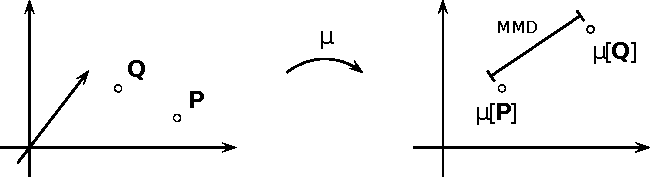
\includegraphics[width=0.8\textwidth]{geometric_mean_embedding.pdf}
\clearpage

\subsection*{HSIC as MMD}
\textbf{Notation}
$(X,Y)$ random vector taking values in the product space $(\mathcal{X},\mathcal{Y})$, and define the kernel on $(\mathcal{X},\mathcal{Y})$ via
\begin{align*}
&\mathcal{X}\times\mathcal{Y}\rightarrow\mathbb{R}\\
&((x,y),(\tilde x,\tilde y))\mapsto k(x,\tilde x)\cdot \ell (Y,\tilde Y)
\end{align*}
where $k(\cdot,\cdot),\ell(\cdot,\cdot)$ are kernels on $\mathcal X,\mathcal Y$ resp.

\clearpage

\subsection*{HSIC as MMD}
MMD for the distributions $\mathbb P:=\mathbb{P}^{(X,Y)}$ and $\mathbb Q:=\mathbb{P}^{X}\otimes\mathbb{P}^{Y}$ can be expressed as
\begin{equation*}
\text{MMD}(\mathbb{P}^{(X,Y)},\mathbb{P}^{X}\otimes\mathbb{P}^{Y})^2=\text{HSIC}(\mathbb{P}^{(X,Y)})
\end{equation*}
Proof: on the board.

\clearpage

In conclusion:
\begin{align*}
X,Y\; \text{independent}&\Leftrightarrow\;\mathbb{P}^{(X,Y)}=\mathbb{P}^{X}\otimes\mathbb{P}^{Y}\\&\Leftrightarrow\;\text{MMD}(\mathbb{P}^{(X,Y)},\mathbb{P}^{X}\otimes\mathbb{P}^{Y})=0\\&\Leftrightarrow\;\text{HSIC}(\mathbb{P}^{(X,Y)})=0
\end{align*}

\clearpage


%#### Ambra's part
\section{Independence Test based on HSIC}
\clearpage
Let $(X_1,Y_1), \ldots, (X_m,Y_m)$ be independent and identically distributed according to $\mathbb{P}^{(X,Y)}$. We want to test the hypothesis
\newcommand{\indep}{\begin{sideways}%
    $\vDash$\end{sideways}}
\newcommand{\dep}{\begin{sideways}%
    $\nvDash$\end{sideways}}
\begin{equation*}
\begin{matrix}
H_0: & X \indep Y & \mbox{ against} \\
H_1: &  X \dep Y &
\end{matrix}
\end{equation*}

with a significance level $\alpha$ by using the HSIC.

\clearpage

Construction of the independence test:
\begin{enumerate}
\item Use HSIC as test statistics
\item Determine its distribution under $H_0$
\item Find the acceptance region and the decision function of the test
\end{enumerate}

\clearpage

\subsubsection{Step 1: Test statistics based on the HSIC}
Idea: Use the sample estimator of the HSIC obtained by plugging the empirical distributions into 
\begin{align*}
HSIC(\mathbb{P}^{(X,Y)})= & \mathbb{E}_{X,Y}\mathbb{E}_{\tilde{X},\tilde{Y}}k(X,\tilde{X})\ell (Y,\tilde{Y}) \\ &-2 \mathbb{E}_{X,Y}\mathbb{E}_{\tilde{X}}\mathbb{E}_{\tilde{Y}}k(X,\tilde{X})\ell (Y,\tilde{Y}) \\ & +\mathbb{E}_{X} \mathbb{E}_{Y}\mathbb{E}_{\tilde{X}}\mathbb{E}_{\tilde{Y}} k(X,\tilde{X})\ell (Y,\tilde{Y})
\end{align*}

\clearpage

the result is the V-statistic

\begin{align*}
\widehat{HSIC} = & \frac{1}{m^2} \sum^{m}_{i,j=1} k(X_i,X_j) \ell (Y_i, Y_j) \\
& - 2\frac{1}{m^3}\sum^{m}_{i,j,f=1} k(X_i,X_j) \ell (Y_i, Y_f)  \\ & + \frac{1}{m^4}\sum^{m}_{i,j,f,g=1} k(X_i,X_j) \ell (Y_f, Y_g)
\end{align*}

\clearpage

which is equivalent to 
\begin{equation*}
\widehat{HSIC} = \frac{1}{m^2} \mbox{trace} (KHLH)
\end{equation*}

where

\begin{align*}
(K)_{ij} = & k(X_i, X_j) \\
(L)_{ij} = & \ell (Y_i,Y_j)  \\
H= & Id_m - \frac{1}{m}\mathbf{1}\cdot \mathbf{1^t}
\end{align*}


\clearpage

\subsubsection{Step 2: Distribution of $\widehat{HSIC}$ under $H_0$}

\textbf{Theorem} Under the assumption of independence we have

\begin{equation*}
m\cdot\widehat{HSIC} \overset{\text{\scriptsize d}}{\rightarrow} 6\cdot \sum^{\infty}_{p=1} \lambda_p \omega_p^2
\end{equation*}
where $\omega_j^2 \overset{\text{\scriptsize iid}}{\sim}  \chi_1^2$ and $\lambda_p$ solves the eigenvalue problem
\begin{equation*}
\lambda_p g_p(z_j) = \int h_{ijqr} g_p(z_i) d\mathbb{P}^{(Z_i, Z_q, Z_r)}
\end{equation*}
where 
\begin{align*}
Z_j= &(X_j,Y_j) \\
h_{ijqr}= &\frac{1}{4\!}\sum_{(t,u,q,r)\in\mathbb{S}}k_{tu}\ell_{tu} + k_{tu}\ell_{vw}-2k_{tu}\ell_{tv}
\end{align*}
Note that $\mathbb{S}$ indicates the set of all ordered quadruples drawn without replacement from $(i,j,q,r)$.
\clearpage

But the complexity of both the eigenvalue problem and the sum over a large number of random variables makes difficult to get the exact quantiles.
\clearpage

Trick (Kankainen): Use a Gamma Approximation:
\begin{equation*}
m \cdot \widehat{HSIC} \overset{\text{\scriptsize d}}{\thickapprox} \Gamma(\gamma, \beta)
\end{equation*}

where 
\begin{align*}
\gamma &= \frac{(\mathbb{E} \widehat{HSIC})^2}{var \widehat{HSIC}} \\
\beta & = m\cdot \frac{var\widehat{HSIC}}{\mathbb{E}\widehat{HSIC}}
\end{align*}
\clearpage

Note: To compute the moments efficiently we use, again, an approximation.
\begin{align*}
\mathbb{\widehat{E}} = & {\color{ETHlightgray} \frac{1}{m} + \frac{1}{m^4(m-1)^2}\sum_{i<j}k_{ij}\sum_{i<j}\ell_{ij}-\frac{1}{m^2(m-1)}\sum_{i<j}k_{ij}} \\& {\color{ETHlightgray} - \frac{1}{m^2(m-1)}\sum_{i<j}\ell_{ij} }\\
\widehat{var} & = {\color{ETHlightgray}\frac{2(m-4)(m-5)}{m(m-1)(m-2)(m-3)} \mathbf{1^{t}}(B-diag(B))\mathbf{1}}
\end{align*}

where $B=((HKH).\cdot (HLH)).^2$

\clearpage

\subsubsection{Step 3: Acceptance region and decision function}

Recall: $HSIC(\mathbb{P}^{(X,Y)})$ ''measures the distance between $\mathbb{P}^{(X,Y)}$ and $\mathbb{P}^X \otimes \mathbb{P}^Y$''.\\

Then the acceptance region has the form

\begin{equation*}
\left[ 0, c\right]
\end{equation*}

where the threshold $c$ corresponds to the $(1-\alpha)$ quantile of $\Gamma(\gamma,\beta)$.

\clearpage

Then the decision function has the form

\begin{equation*}
d\left((X_1,Y_1), \ldots, (X_m, Y_m)\right)=\left\lbrace\begin{matrix}
H_0, & \widehat{HSIC}\leq c \\
H_1, & \widehat{HSIC} > c
\end{matrix} \right.
\end{equation*}

\clearpage
\section{In practice}
\begin{wrapfigure}{l}{0.5\textwidth}
  \begin{center}
    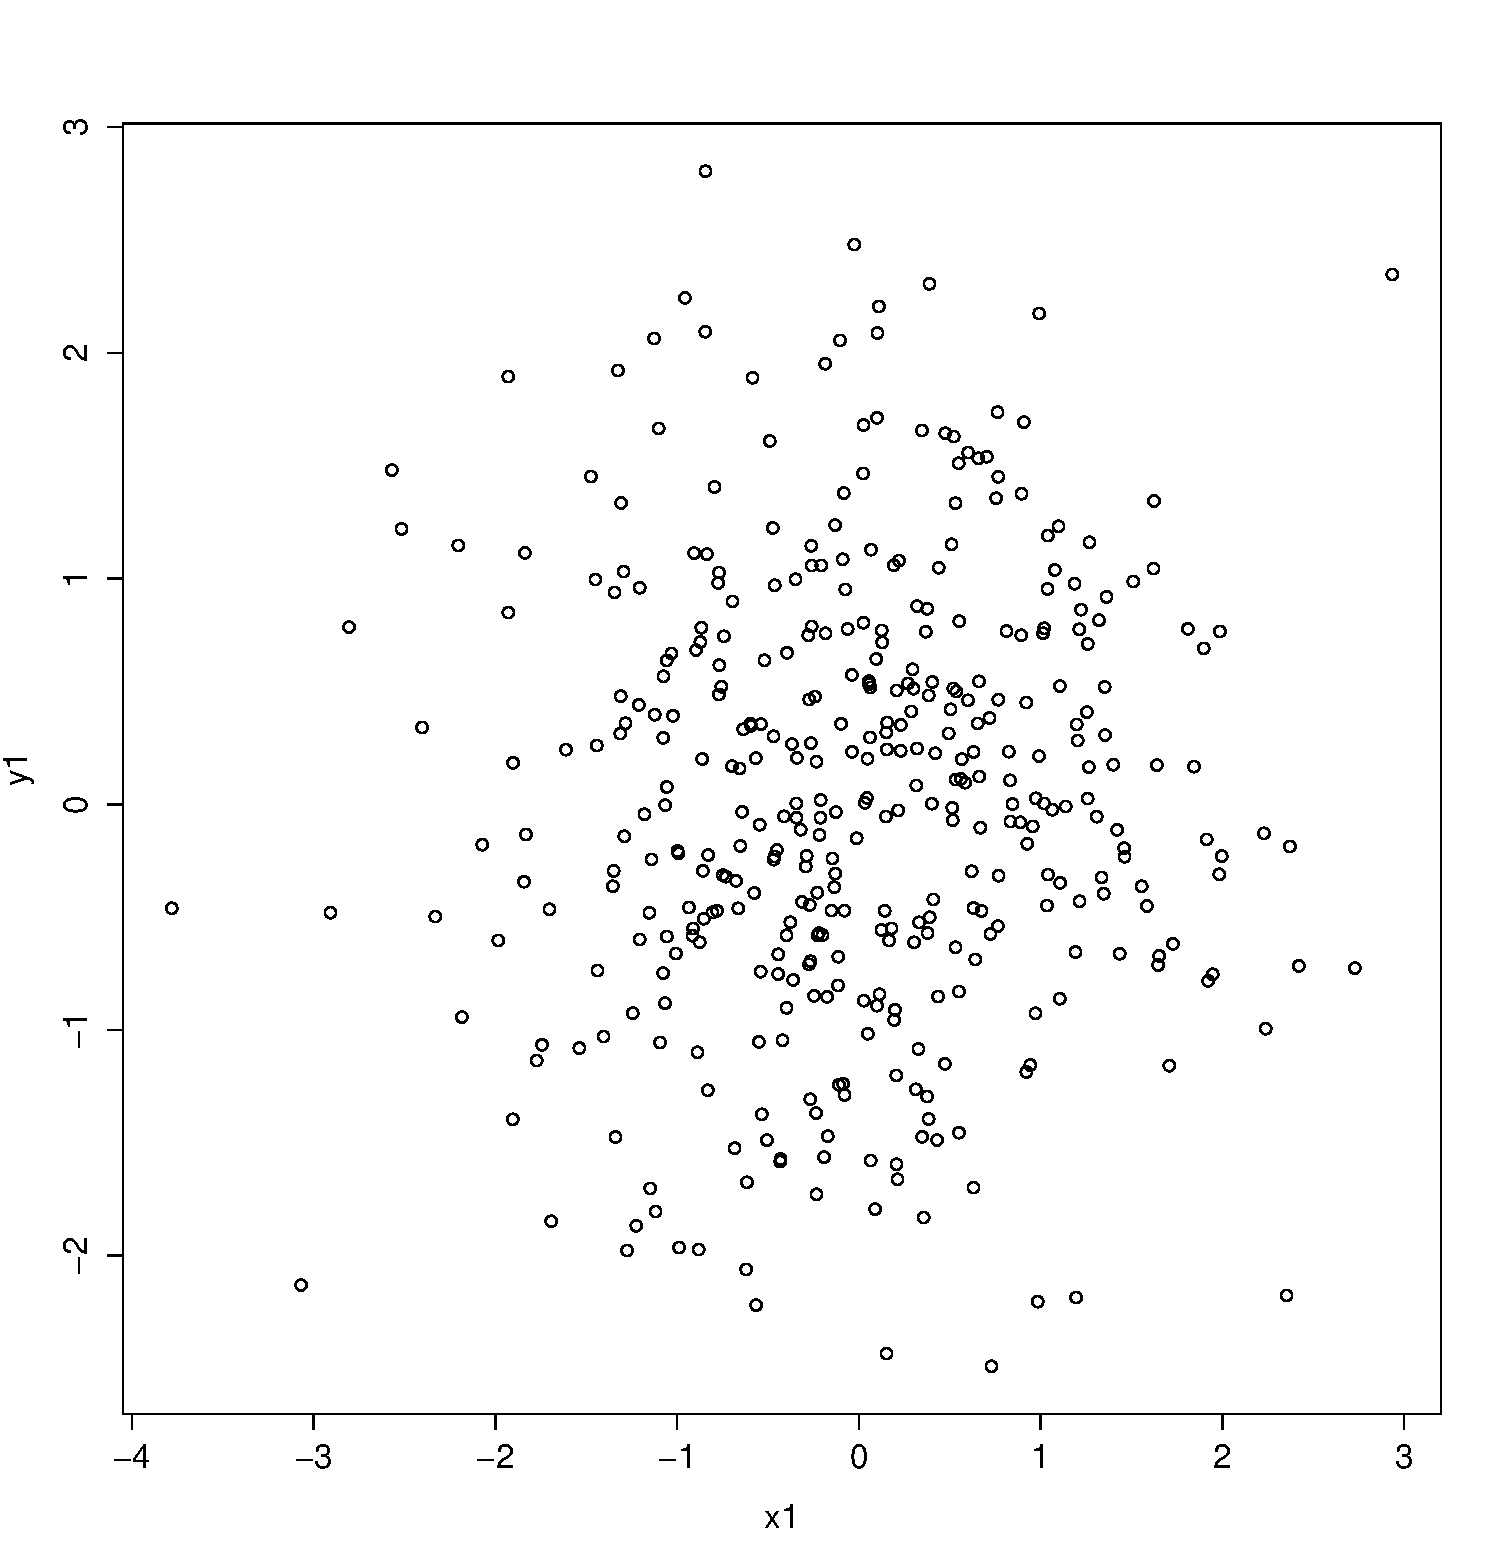
\includegraphics[width=5cm]{x1_vs_y1.pdf}
  \end{center}
\end{wrapfigure}
$H_0$: $\HSIC(x_1, y_1)=0$.

$H_A$: $\HSIC(x_1, y_1)\ne0$.

$P_0 = 0.54$

\clearpage
\begin{wrapfigure}{l}{0.5\textwidth}
  \begin{center}
    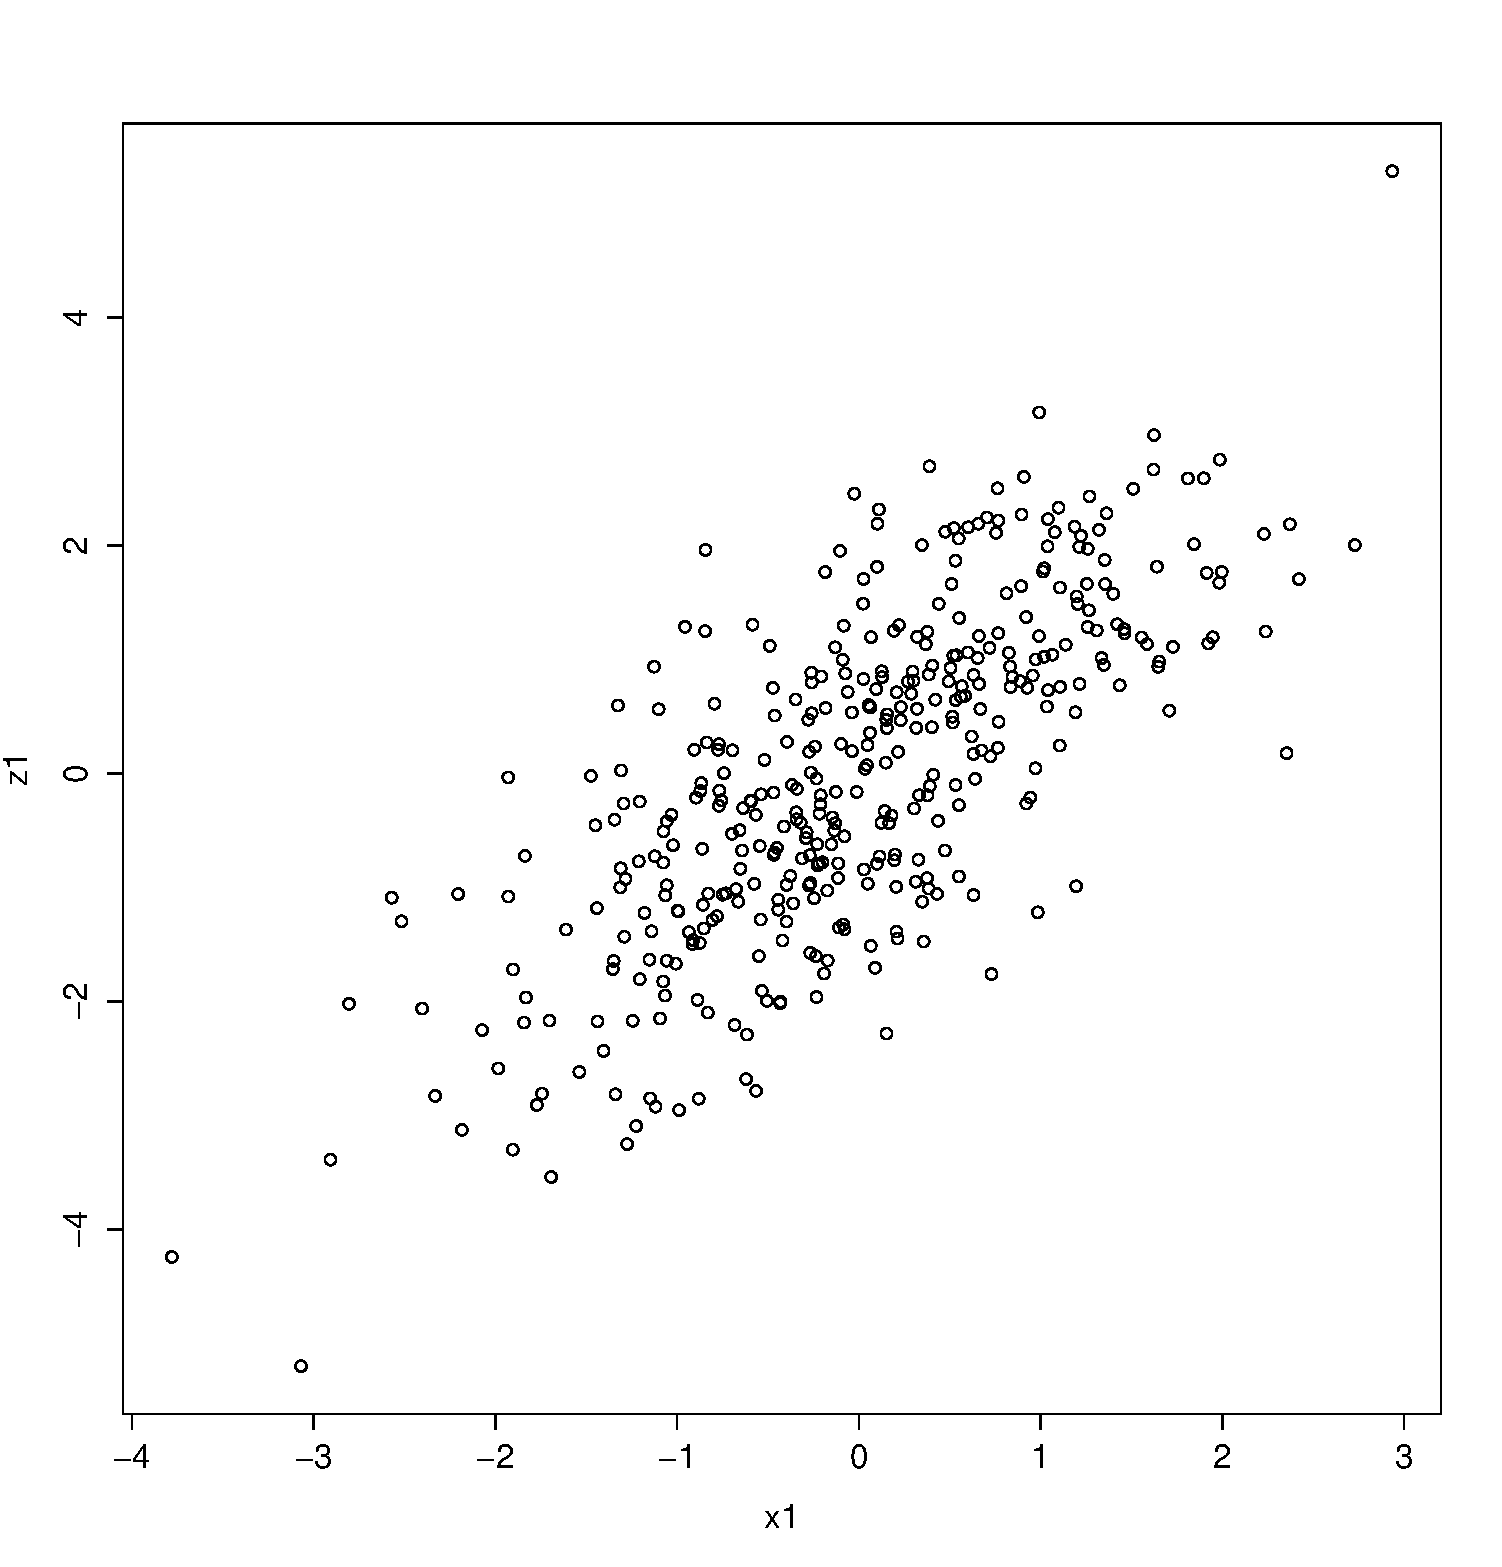
\includegraphics[width=5cm]{x1_vs_z1.pdf}
  \end{center}
\end{wrapfigure}
$H_0$: $\HSIC(x_1, z_1)=0$.

$H_A$: $\HSIC(x_1, z_1)\ne0$.

$P_0 = 0.0$
\clearpage
\begin{wrapfigure}{l}{0.5\textwidth}
  \begin{center}
    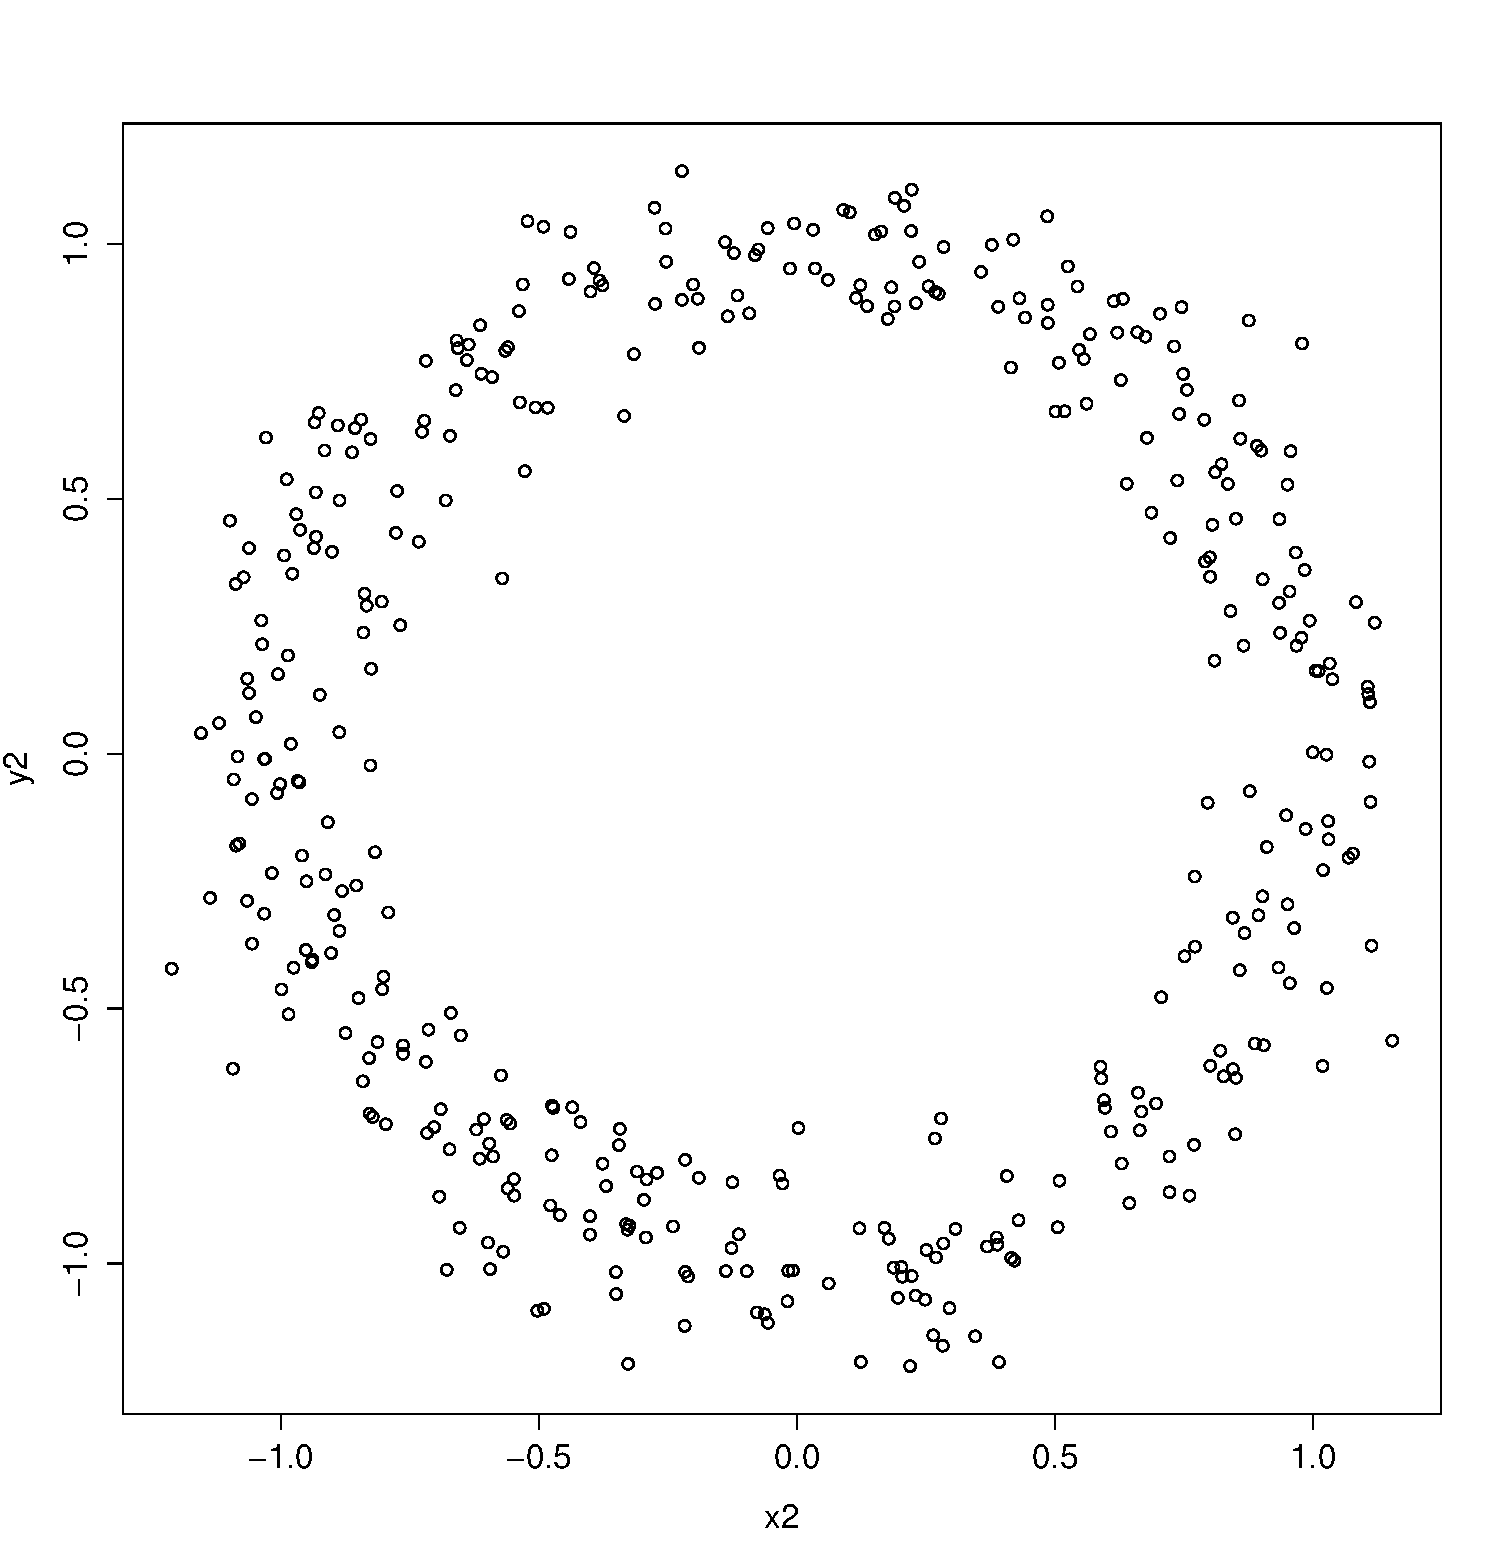
\includegraphics[width=5cm]{x2_vs_y2.pdf}
  \end{center}
\end{wrapfigure}
$H_0$: $\HSIC(x_1, z_1)=0$.

$H_A$: $\HSIC(x_1, z_1)\ne0$.

$P_0 = 0.0$
\clearpage

% ===== special page ===========================================================
% ===== page with a background picture =========================================
%\ThisCenterWallPaper{1}{ETH_res/ETH_neutral.jpg}
\ThisCenterWallPaper{1}{ETH_neutral.jpg}
\textcolor{white}{ % change the text on the background picture to white
Biblography
\begin{itemize}
	\item Gretton et al. \emph{A Kernel Statistical Test of Independence}, NIPS 2007
	\item Peters. \emph{Asymmetries of Time Series under Inverting their Direction}. Diploma Thesis. 2008. \emph{(Some diagrams reproduced from this work.)}
\end{itemize}
}


%\ifoot{}% switch off the i-footer for this page used in ETH_res/ETH_settings.tex
\ifoot{}% switch off the i-footer for this page used in ETH_settings.tex
\clearpage
%% ===== page after a background picture page ==================================
%\ifoot{% switch on the i-footer for all following pages again
%	\hspace{-6.0mm}
%    \vspace{-8.5mm}
%	\begin{tikzpicture}[remember picture,overlay]
%		\node [xshift=\paperwidth/2,yshift=\footheight/2]
%%        {
\includegraphics[width=\paperwidth]{ETH_res/ETH_footer.jpg}};
%        {
\includegraphics[width=\paperwidth]{ETH_footer.jpg}};
%	\end{tikzpicture}
%}%
%
%% now on normal text again
%More discussion 

\end{document} 